%\RequirePackage[l2tabu, orthodox]{nag} %Package complains about uses of old functions, make sure you write modern latex
\documentclass[letterpaper,10pt]{report}
\usepackage[english,canadian]{babel}
\usepackage{amsmath} %AMS Math Package
\usepackage{amssymb} %AMS Math Symbols
\usepackage[all,warning]{onlyamsmath}%Warn about non-ams math useage, suggest improvements
\usepackage[letterpaper,top=1.5in,left=1.5in,bottom=1in,right=1in]{geometry} %Sets up basic page dimensions
\usepackage[newcommands]{ragged2e} %provides better \right \left and \Centering, replaces old commands with improved ones
\usepackage[tracking=true,kerning=true,expansion]{microtype} %makes type look better
\usepackage{booktabs} %makes tables look better
\usepackage{siunitx} %provides standard printing for SI units
\usepackage[breaklinks,hidelinks]{hyperref} %Provides clickable links
\usepackage{cleveref} %Allows use of \cref, which knows what kind of ref you're making, so you don't have to write EQN and such
\usepackage{ifpdf} %Conditions for if pdftex is running
\usepackage[T1]{fontenc} %upgrades font encodings
\usepackage[utf8]{inputenc}%Tells latex the file is saved as UTF-8 (make sure it is!)
\usepackage{lmodern} %improved version of computer modern font
\usepackage{multirow} %Allows for mulirow a.k.a. grouped cells in tables
\usepackage{fixltx2e} %Fixings bugs in latex2e that aren't fixed due to breaking backwards compatability
\usepackage{upgreek} %Provides upright (non italic) greek fonts
\usepackage{gensymb} %Provides  \de­gree, \cel­sius, \pert­hou­sand, \mi­cro and \ohm amongst others
\usepackage{textcomp}
\usepackage{textgreek} %Provides \textbeta and similar greek letters in text mode
%\usepackage[section]{placeins} %Fixes placement of figures so they don't cross section boundaries
\usepackage[section,subsection,subsubsection]{extraplaceins} %Modified version of placeins which works at section, subsection and subsubsection
\usepackage{verbatim}%Fixes bugs in \verbatim, and provides \begin{comment} and \verbatiminput for including files
\usepackage{syntonly}%Provides syntax-only latex runs, useful for when the document starts getting big!
\usepackage{csquotes}
\usepackage{float} %Fixes up floats (figures) and provides the H placement modifier (place the float RIGHT HERE). with great power...
\usepackage[style=nature,backend=bibtex]{biblatex}
%\addbibresource{library.bib}
\usepackage[english]{isodate}%Convert any date formats to ISO style
\usepackage{listing}%Package for listing sourcecode with syntax highlighting
\usepackage{ellipsis}%Fix \ldots and similar commands, bugs with spacing and such
\usepackage{graphicx}
\usepackage{wasysym}

\pdfminorversion=5
\pdfobjcompresslevel=3 
\pdfcompresslevel=9

\usepackage{subcaption} %The standard method to do figures with a), b) and such
\usepackage{fancyhdr} %Package for changing header/footer
\usepackage{showkeys} %Prints all instances of \label in margin for easy writing
\usepackage{lineno} %Allows labeling of line numbers throughout document
\usepackage{makeidx} %For generating index files
\usepackage{lipsum} %Prints junk text with \lipsum
\usepackage{setspace} %Provides \doublespacing command
\usepackage{todonotes} %Provides \todo{something} which puts labels in magin and \missingfigure{something} to put in placeholder figures

\widowpenalty=300 %Prevent widows (single sentences at end of page)
\clubpenalty=300 %Prevent orphans (single sentences on empty pages)
%\doublespacing %Uncomment to turn on double spacing
%\linenumbers %Uncomment to turn on line numbers
%\syntaxonly %Uncomment to only check compile for syntax PRODUCES NO OUTPUT

\hypersetup{
    unicode=true,          % non-Latin characters in Acrobat’s bookmarks
    pdftoolbar=true,        % show Acrobat’s toolbar?
    pdfmenubar=true,        % show Acrobat’s menu?
    pdffitwindow=false,     % window fit to page when opened
    pdfstartview={FitH},    % fits the width of the page to the window
    pdftitle={My title},    % title
    pdfauthor={Gabriel A. Devenyi},     % author
    pdfsubject={Subject},   % subject of the document
    pdfkeywords={keyword1} {key2} {key3}, % list of keywords
    pdfnewwindow=true,      % links in new window
    colorlinks=false,       % false: boxed links; true: colored links
    linkcolor=red,          % color of internal links
    citecolor=green,        % color of links to bibliography
    filecolor=magenta,      % color of file links
    urlcolor=cyan           % color of external links
}
\graphicspath{{figures/}} %Uncomment if you want to hide all figure files in a graphics/ subdirectory


\title{Thesis Example}
\author{Gabriel A. Devenyi}
\date{\today}

\makeindex

\begin{document}

\begin{titlepage} %Half-title page for McMaster Formatting
	\vspace*{\fill}\Centering
	Energy and Symmetry at Surfaces: Role in Nanostructures and Epitaxy
	\vspace*{\fill}
\end{titlepage}
% % % % % % % % % % % % % % % % % % % % % % % % % % % % % % % % % % % % % %
\begin{titlepage} %Titlepage
\Centering
\vspace*{\fill} %This makes text vertically centered
{\Large ENERGY AND SYMMETRY AT SURFACES:\\ROLE IN NANOSTRUCTURES AND EPITAXY\\
By\\GABRIEL A.\ DEVENYI, B.\ ENG.\\}
\vfill 
A Thesis Submitted to the School of Graduate Studies in Partial Fulfilment of 
the Requirements for the Degree Doctor of Philosophy
McMaster University
\vfill%This pushes copyright to the bottom
\textcopyright Copyright by Gabriel A.\ Devenyi, May 2013
\end{titlepage}
% % % % % % % % % % % % % % % % % % % % % % % % % % % % % % % % % % % % % %
\pagenumbering{roman}
\setcounter{page}{2} %Descriptive note page
{\Large Descriptive Note\\
DOCTOR OF PHILOSOPHY (2013) McMaster University
(Engineering Physics)
Hamilton, Ontario
TITLE: The Character and Administration of Governor John Wentworth\\
AUTHOR: Gabriel A. Devenyi, B.\ Eng. (McMaster University)\\
SUPERVISOR: Professor John S. Preston\\
NUMBER OF PAGES: vii, 212}
% % % % % % % % % % % % % % % % % % % % % % % % % % % % % % % % % % % % % %
	\begin{abstract}
		\thispagestyle{plain}
		\setcounter{page}{3}
			Abstract goes here.
	\end{abstract}
% % % % % % % % % % % % % % % % % % % % % % % % % % % % % % % % % % % % % %
	\setcounter{page}{4}
	\chapter*{Acknowledgements}
	My wife, my dog, my parents, my supervisor.
	\newpage

	\tableofcontents
	\listoffigures
	\listoftables
	\newpage
	\pagenumbering{arabic} %Reset page numbering

%Fix all the header/footer according to McMaster Requirements
	\fancypagestyle{plain}{
	\fancyhf{}
	\lhead{PhD Thesis - Gabriel A.\ Devenyi}
	\chead{}
	\rhead{McMaster University - Engineering Physics}
	\cfoot{\thepage}}
	\pagestyle{fancy}
	\fancyhead{}
	\lhead{PhD Thesis - Gabriel A.\ Devenyi}
	\chead{}
	\rhead{McMaster University - Engineering Physics}
	\cfoot{\thepage}

% % % % % % % % % % % % % % % % % % % % % % % % % % % % % % % % % % % % % %
%Thesis starts here

%For large LaTeX documents, it is best practice to separate the material into smaller files so that it is easier to handle, use \input to insert each file into the overall document

%Epitaxy has been a dominant technological feature since near the very inception of the semiconductor age.
It has also been intimately entwined with the dominant semiconductor up till the present day, silicon.
Silicon has dominated almost every field of semiconductor research for the better part of 40 years, becoming the most well understood material in the world.
This vast focus on silicon has also greatly influenced the thinking of what were at the time fledgling fields, most notably epitaxy.
\emph{Epi-taxis} or ``above --- in an ordered manner'' is the Greek root of the term epitaxy and as it is originally defined, it has been very narrowly interpreted by most of the research field.
Silicon on silicon epitaxy, or homoepitaxy, has been the dominant type of epitaxy both for research and production, due to its relevance to semiconductor chip manufacturing.
This idea of the `ideal' epitaxy as modelled by silicon homoepitaxy has pervaded the thinking of research into the field, with the material systems being most similar as the result being the most researched, and the most successful.

The material systems most similar to homoeptiaxy (besides other homoepitaxy) are the III-V group semiconductors, specifically the Al/Ga/In-P/As/Sb binary/ternary/quaternary family as in \cref{fig:intro_bandgaps}.
These zincblende semiconductors through the manipulation of exact atomic concentration, can be grown from exactly lattice matched to strongly mismatched. These material systems all have covalent or primarily covalent bonds with strongly preferred atomic sites for the atomic species.
When parameters are optimized, epitaxial growth in such systems is orientationally commensurate with the underlying substrate and dominated by strain effects.
\begin{figure}
    \centering
    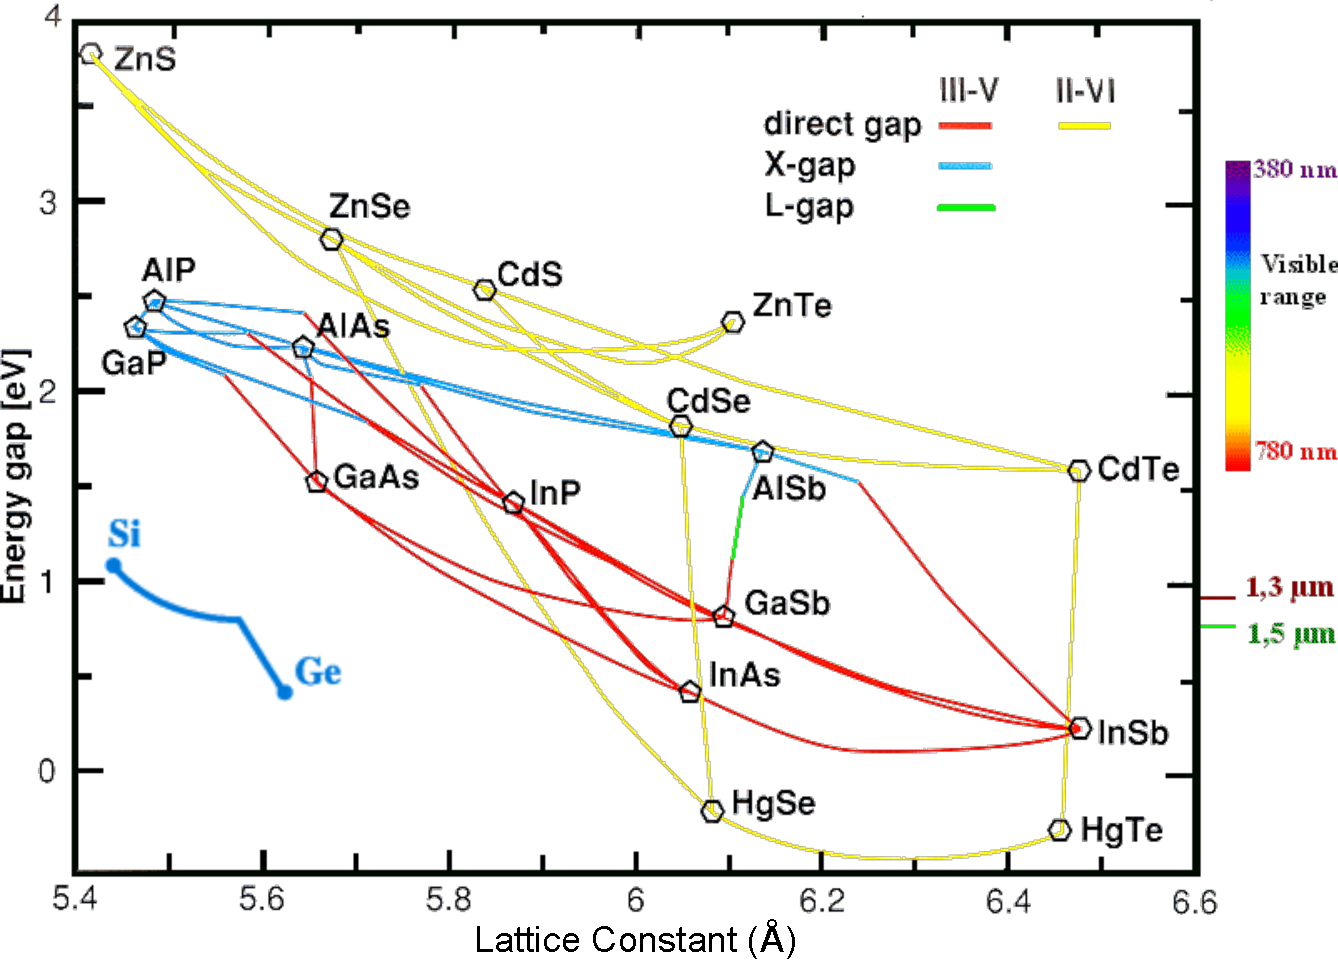
\includegraphics[width=0.9\textwidth]{intro_bandgaps}
    \caption[Bandgap versus lattice constant]{\label{fig:intro_bandgaps}Bandgap versus lattice constant for the most common semiconductors (modified from Helmut\cite{HelmutFoll2013}) (used with permission)}
\end{figure}

Beyond the III-V homologous growth systems, the next most investigated epitaxial process is when these materials are grown on silicon.
In addition to the always-present issue of strain due to the intrinsic lattice mismatch between the III-V family and silicon, the diamond structure of silicon results in an issue of polar (zincblende) on non-polar (diamond) epitaxy\cite{Kroemer1987} where group III and group V atoms cannot differentiate between sites on the silicon surface.
Such site non-specificity has been an issue of great interest to the epitaxy research community resulting in numerous attempts (some successful)\cite{Kroemer1987} to improve growth of such a chemically dissimilar system.

Outside the extensive research into the epitaxy of silicon and the III-V systems, work into epitaxy has mostly been on a material-by-material basis.
Material systems of interest are examined on an issue by issue basis with the goal of producing high quality material for some application, rather than examining the generalized epitaxy phenomenon.
In this work, the goal has been to expand the understanding of epitaxy through an experimental exploration of several model systems which are epitaxial corner cases, and to show other conditions under which high quality epitaxy can occur.
Through this work, two key themes were examined in epitaxial systems, the role of symmetry and the role of energy at epitaxial interfaces.
These themes were examined through investigations into three model material systems, III-V semiconductors on silicon, II-VI semiconductors on crystalline oxides, and noble metals on crystalline oxides.
Investigations into III-V semiconductors on silicon focused on the role of vicinal surfaces, surface reconstructions, and higher order crystal surfaces. Vicinal (or offcut) surfaces of substrates, truncated and reconstructed, were found to have a strong effect on twinning during epitaxial growth, a potential method of improving quality of material growth. (211), a higher order substrate orientation was found to allow accommodation of strain by tilting of a growing epitaxial layer.
Investigations into II-VI semiconductors concentrated on the role of surface reconstructions, and the role of bond strength in epitaxial interfaces. A new epitaxial relationship between temperature stable surface reconstruction and CdTe was observed and atomically modeled, such stable surface reconstructions may offer a new route for lattice matched epitaxial growth. In addition, growths of CdTe on sapphire substrates were found to show a unique liftoff phenomenon, where single crystal films are weakly bonded to the substrate and can be removed while maintaining crystalinity.
Finally, investigations into noble metals on oxide surfaces concentrated on the properties of epitaxy in the weak bonding regime. Epitaxial growth of gold on spinel, a complex oxide, was found to be possible, despite the weak reactivity of both the noble metal and the oxide substrate.
The results from these investigation and the main contribution of this work is to show that epitaxy is possible for symmetrically and chemically dissimilar model systems, and to experimentally examine the implications to epitaxy that such systems have.

\section{Major Themes}
\subsection{Symmetry}
The 2D (and as we shall later see sometimes 3D) interface that separates the epitaxial substrate from the growing crystal has a symmetry relationship which relates the substrate to the crystal.
These surface symmetries are different than the bulk symmetry of the substrate and crystal.
In the simplest treatment of surfaces, the surface of a given substrate is simply a truncation of the crystal in a given orientation, exposing a plane of atoms which then present a subsymmetry of the bulk crystal. Any truncation through a bulk crystal is unstable, since the surface is now exposed to the outside world, and the surface can resolve this instability in a variety of ways.
As will be seen later there are many complications to this model and it is in these complications that we find interesting changes in symmetry, breaks in symmetry and distortions of this 2D surface into a more complex 3D interface.
It is these changes to the surface symmetry, and it's interaction with the growing crystal which have profound and useful implications for epitaxy.
The first major theme investigates the implications of unique interface symmetries, broken symmetries and 3D interfaces on the epitaxial process.

\subsection{Energy}
While symmetry describes the spatial distribution of the landscape presented to a growing crystal, energy describes the magnitude of the effect that landscape has.
Strong energy landscapes cause the symmetry of a given substrate to have it's influence felt strongly, while a weak landscape can have a subtle effect on growth. Whether atoms are bonded via physisorption, covalent bonding, ionic attraction or Van der Walls forces determines the strength of the interface landscape energy.
The energy landscape of the epitaxial interface can vary over a large range, and the role of these strengths has not been examined extensively.
The second major theme of this work investigates the implications of energy landscapes outside the typical heteroepitaxy regime, specifically relating to the weaker energies.

\section{Secondary Themes}
\subsection{Combined Reciprocal Space and Real Space Characterization}
The investigations into epitaxy discussed throughout this thesis have relied upon a variety of techniques to reveal the patterns behind these processes. The most fruitful of the techniques utilized in this work has been the combined use of reciprocal space mapping via 2DXRD and the direct imaging of samples using TEM/STEM. These techniques, when used individually, often lead to ambiguity in the results. STEM/TEM, being a small-area sampling technique can frequently miss information, or cause false interpretations of ``common'' results, when a given sample may be unique or atypical. Similarly, the use of reciprocal space mapping alone gives a picture which convolves all of the data in the sampling area together, providing little insight about its spatial distribution. When these two techniques are combined, the two datasets must be successfully reconciled for a given model of the underlying system to be coherent. Such consistency requirements allow competing explanations to be discriminated from one another based on predictions they make about the data, leading to more complete and less ambiguous models. Such a combination of techniques has also encouraged collaboration, as one cannot be an expert in the operation and interpretation of both systems without compromising the work one originally intended to do.

\chapter{The Role of Vicinal Surfaces in Epitaxial Twin Formation}
%\subsection{Introduction}
Since the microelectronics revolution, Silicon has been a dominant material 
for the production of devices for a variety of applications. Silicon has 
non-ideal properties for a variety of applications but remains dominant due 
to its well-understood processing parameters and large manufacture install 
base, providing economies of scale. The III-V semiconductors offer superior 
properties for a variety of applications when compared to silicon, and are 
actively used in applications were performance is valued above other 
considerations, such as military and space sectors. The goal of integrating 
III-V semiconductors into silicon based microelectronics has spawned extensive 
research into the processing involved to grow or otherwise electronically 
attach these materials with minimal defects.

Under auspices of the ARISE Photovoltaics project, the III-V 
semiconductors GaAs, GaSb, AlSb and InP were grown as thin films under a 
variety of conditions on single crystal silicon substrates, in order to 
examine the growth process and electro-optic properties. The role of the 
varied lattice mismatch, growth parameters, and substrate properties were 
examined and several previously undocumented phenomona were examined due to 
the use of 2DXRD, whose benefits were documented in \cref{sec:2DXRD}.

The formation of epitaxial (or growth) twins was found to be a key area where 
the literature had performed little examination. The role of twins in the 
formation of electronic defect networks, and the effects vicinal (offcut) 
substrates had on their formation were thoroughly examined and a 
explanatory model was developed to explain factors that affect their formation 
and provide proposed routes towards their minimization and 
elimination\cite{Devenyi2011}. This work was completed in close collaboration 
with Ms. Steffi Woo, a Ph.D. candidate in Material Science and Engineering and 
McMaster, with the TEM/STEM work performed exclusively by her and all other 
work being collaborative.

\subsection{Background}
\todo{Should a section covering the background of III-V on Silicon go here, or 
go into the introductory material at the beginning of the thesis}

\subsection{Experimental} \todo{This section is currently copy-pased from 
paper, is this appropriate?}
Semiconductor thin films (GaAs, InP, GaSb, and AlSb) were deposited on nominal 
(001)-oriented ($\pm$0.5$^\circ$) and vicinal Si substrates (offcut 
4.7$^\circ$ ($\pm$0.25$^\circ$) towards [110]) using a SVT Associates 
molecular beam epitaxy (MBE) system. As-received epi-ready wafers were cleaned 
for 1 min in a 4\% HF in deionized (DI) water dip followed by a 30 sec DI 
rinse immediately prior to their insertion into the MBE load-lock. Before film 
deposition, both the nominal and vicinal Si(001) substrates underwent a 15 min 
degassing procedure at 350~$^\circ$C followed by a thermal treatment at 
800~$^\circ$C for up to 5 min, in order to reconstruct the Si surface into 
single domain 
terraces\cite{NeergaardWaltenburg1995,S1991,Sakamoto1986,Pehlke1991}. A small 
number of single steps are expected to remain on vicinal substrates, a higher 
number on nominal substrates because of the larger terrace length. Growth 
conditions followed established 
protocols\cite{Akahane2004,Balakrishnan2006a,Fischer1986} and yielded 
comparable rocking curve full-width half-maximum for the [004] reflection 
using double crystal X-ray diffraction. AlSb thin films were grown to a 
thickness of 550~nm with a 20~nm GaSb capping layer to avoid oxidation. GaAs 
thin films was grown to a thickness of 600~nm and GaSb to a thickness of 
500~nm. InP samples were grown at 470~$^\circ$C with a V/III flux ratio of 2 
at a growth rate of 1 $\mu m$/hr, resulting in a thickness of 600~nm. Double 
crystal X-ray and TEM data also revealed that all films are fully relaxed by a 
network of interfacial misfit dislocations\cite{Vajargah2011}. GaSb samples 
were grown in the presence of a 5 nm AlSb buffer layer, as prescribed by 
Akahane \textit{et al}.\cite{Akahane2004}.

Stereographic pole figures were generated for each sample using 2DXRD 
techniques. A Bruker SMART 6000 CCD detector on a Bruker 3-circle D8 
goniometer (Bruker AXS Inc., Madison, WI) with a Rigaku RU-200 rotating anode 
X-ray generator (Rigaku MSc, The Woodlands, TX) and parallel-focusing 
monochromator optics was used for the data collection. Scans were taken with 
the detector centered on the (111) 2$\theta$ of the material of interest and 
the sample rotated through 360$^\circ$ in 0.5$^\circ$ increments about the 
surface normal of the sample. A 1D integration of all frames was used to 
determine the combined width of the (111) peaks using MAX3D software (McMaster 
University)\cite{Britten2007}. The peak width was then used to integrate (111) 
reflections from all frames, including a background and absorption correction 
for the corresponding material with GADDS (Bruker-AXS) software, resulting in 
a pole figure. Pole intensities were obtained from pole figures using a 
circular integration cursor with a 10 pixel radius which was centered on the 
pole so as to maximize the total intensity captured. All pole intensities were 
corrected for structure factor and frame exposure times.

For each sample two \{110\} TEM cross-sections were prepared, one parallel to 
the [110] miscut direction and the other perpendicular. The specimens were 
prepared by the standard procedure of mechanical polishing, dimpling, and 
ion-milling (4 keV Ar-ions at an incident angle of $\pm$4$^\circ$ using a 
liquid nitrogen cold stage for InP) until perforation. Crystallographic 
information of the epitaxial layer was obtained using diffraction contrast 
imaging with a Philips CM12 conventional transmission electron microscope 
(TEM) operated at 120 kV and equipped with a LaB$_6$ filament. In addition, 
electron diffraction analysis was performed using selected area electron 
diffraction (SAD).
\subsection{Results}
2DXRD measurements performed on as-grown thin films indicated a bulk 
orientation of the material consistent with epitaxial alignment with the 
single crystal silicon substrate. The pole figures generated from 2DXRD data, 
such as \cref{fig:twins_pole_example} also contained a number of other peaks 
at reduced intensity indicating other orientations of the material of interest 
other than the bulk orientation. In order to develop a comprehensive picture 
of the distribution of the grown thin films, simulated pole figures were 
examined in an attempt to generate a composite pole figure which qualitatively 
matched the figures generated from data. Based on these simulations, the 
simulated pole figure \cref{fig:twins_sim_polefigure} was developed, 
indicating that the thin films consisted of a bulk epitaxial phase, and four 
primary twin phases, along with secondary twin phases (not shown). The primary twins form 
along (111), (1$\overline{1}$1) ($\overline{1}\overline{1}$1) and ($\overline{1}$11) 
habit planes.
\begin{figure}
    \begin{subfigure}[b]{0.5\linewidth}
        \centering
        \missingfigure{Representative Single Pole Figure}
        \caption{A representative pole figure of GaAs grown on nominal (100) 
        Silicon\label{fig:twins_pole_example}}
    \end{subfigure}
    \begin{subfigure}[b]{0.5\linewidth}
        \centering
        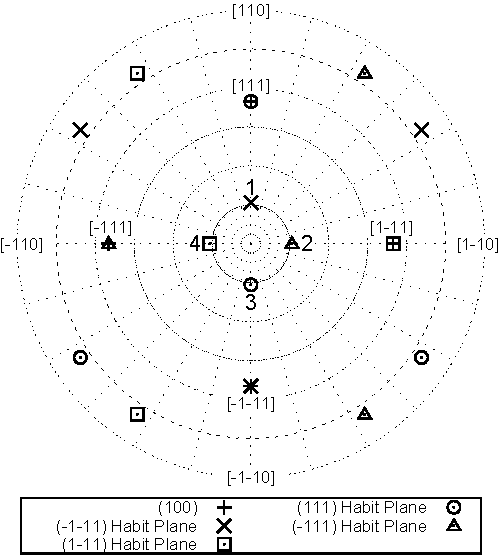
\includegraphics[width=\textwidth]{twins_sim_polefigure}
        \caption{Simulated III-V on silicon pole figure. Unique markers are used 
        for later intensity measurements.\label{fig:twins_sim_polefigure}}
    \end{subfigure}
    \caption{\label{fig:polefigure_example}Represenative pole figure and simulated pole 
    figure}
\end{figure}

Growths of III-V thin films were performed on vicinal substrates due to the established 
literature indicating the ability of atomic height steps formed by such substrates to 
overcome the polar-on-non-polar growth problem\cite{Kroemer1987}. The pole figures 
generated for thin films grown on vicinal substrates were found to have a distinctive 
asymmetry in the intensity distribution of the peaks associated with twinned orientation, 
when compared to the thin films grown on nominal silicon substrates. The pole figures for 
both nominal and vicinal pole figures for the III-V thin films are shown in 
\cref{fig:twins_polefigure}.

\begin{figure}
    \centering
    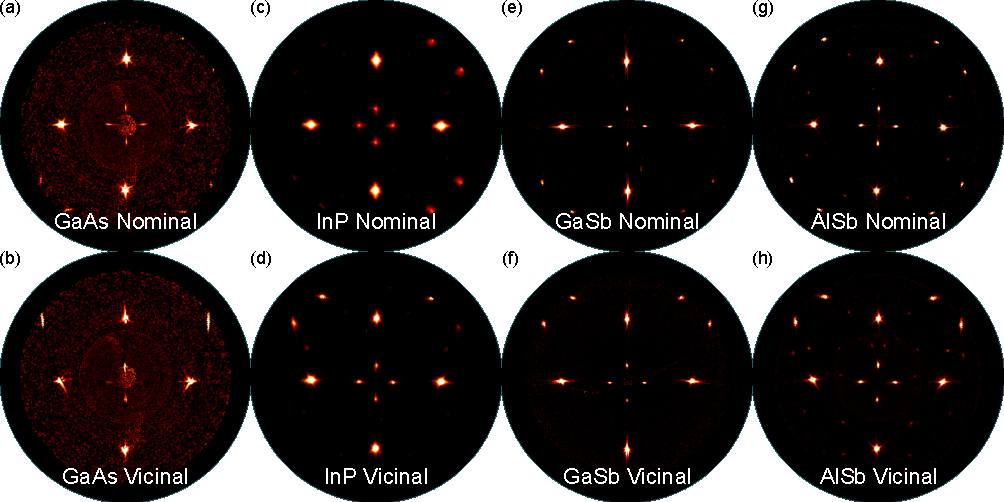
\includegraphics[width=\textwidth]{twins_polefigure}
    \caption{Stereographic \{111\} pole figures generated from 2DXRD show a bulk (100) 
    phase plus four twinned variants as identified in \cref{fig:twins_sim_polefigure}. 
    Twin variant intensity is asymmetric for vicinal 
    substrates.\label{fig:twins_polefigure}}
\end{figure}
\chapter{Tilted Epitaxy on 211 Oriented Substrates}
\section{Introduction}
In parallel to the investigations of vicinal (100) substrates, the ARISE project investigated alternative substrate orientations including (111) and (211). While the results of (111) substrates were uninteresting, growth of thin films on (211) substrates demonstrated a number of interesting properties. Most interesting amongst these was the spontaneous tilting of thin films grown on top of (211) oriented silicon substrates. Such tilting had been remarked upon previously in literature,  but no comprehensive examination of its origins or relationship to material parameters had been examined.

In this work, also done in close collaboration with Ms. Steffi Woo, the spontaneous 
tilting of thin films grown on (211) oriented silicon substrates was examined. The 
effects of the naturally asymmetric substrate was found to cause a tilt of the growing 
thin film in order to minimize the strain across the interface. Using this idea of 
projected strain minimization across the interface, a model was developed which predicted 
the tilt as a function of intrinsic lattice mismatch between the substrate and thin film. 
Examination of the reports of thin film tilting in literature showed the model 
successfully calculated tilt for a large number of material systems and made predictions 
for those systems for which no measured values had been reported.
\section{Background}
The (211) orientation of non-polar semiconductor substrates, most notably silicon, has a number of beneficial properties. Of most relevance to the epitaxy of thin films on Si(211) substrates is the occurrence of two energetically non-equivalent lattice sites on the surface, without the need for surface reconstruction.\cite{Wright1982} These two non-equivalent lattice sites offer preferential nucleation locations for the individual adatoms during growth of polar (group III-V and II-VI) semiconductors. Such preferred nucleation is proposed to eliminate the occurrence of anti-phase domains (APDs) during the growth of polar semiconductors\cite{Wright1982} while also maintaining the interface neutrality condition of h$\pm$k$\pm$l$=$0.\cite{Wright1982} The intrinsic asymmetry of the (211) surface is also expected to influence the formation of epitaxial twins during growth\cite{Devenyi2011}. Si(211) substrates have been used to produce the highest quality CdTe\cite{Zhao2011}, ZnTe\cite{Wang2011a} and HgCdTe\cite{Dhar1997a} despite large lattice mismatches of 19.4\%, 12.3\%, and 19.1\%, respectively. 

Thin films grown on (211) substrates have been previously observed in literature to have a tilted epilayer orientation relative to the substrate.\cite{Zhao2011,Wang2006,Dhar1997a,Lange1991,Nakamura1992} The tilt phenomenon has been attributed to a number of causes by different authors including the glide and interactions of misfit dislocations \cite{Olsen1975,Riesz1994,Ayers1991,Johnson2011} and localized distortion of the lattice at the interface.\cite{Sasaki1992} The mechanisms proposed thus far have been unsuccessful at predicting the tilt of mismatched epilayers over large range of mismatch (0--20\%) found in III-V and II-VI material systems. A phenomenon intimately intertwined with tilted epitaxy is ``dual epitaxy'', observed by numerous authors\cite{Li1995a,Nakamura1992,Rujirawat1998,Lange1991} that mismatched CdTe on GaAs(211) epitaxy can result in films growing in a twinned orientation, combined with a tilt; such that the (133) planes make up the epilayer surface and are parallel to the substrate (211) planes. The tilt component of dual epitaxy is same tilt phenomenon examined here.

\section{Experimental}
GaSb thin films were deposited on nominal (211)-oriented Si substrates, according to our 
previously published procedures\cite{Devenyi2011}, at 600, 640 and 500{\degree}C. Two 
dimensional X-ray diffraction (2DXRD) frames were captured for stereographic pole figure 
analysis and crystallographic indexing as per Devenyi \textit{et al.}\cite{Devenyi2011}.
\begin{figure}
    \centering
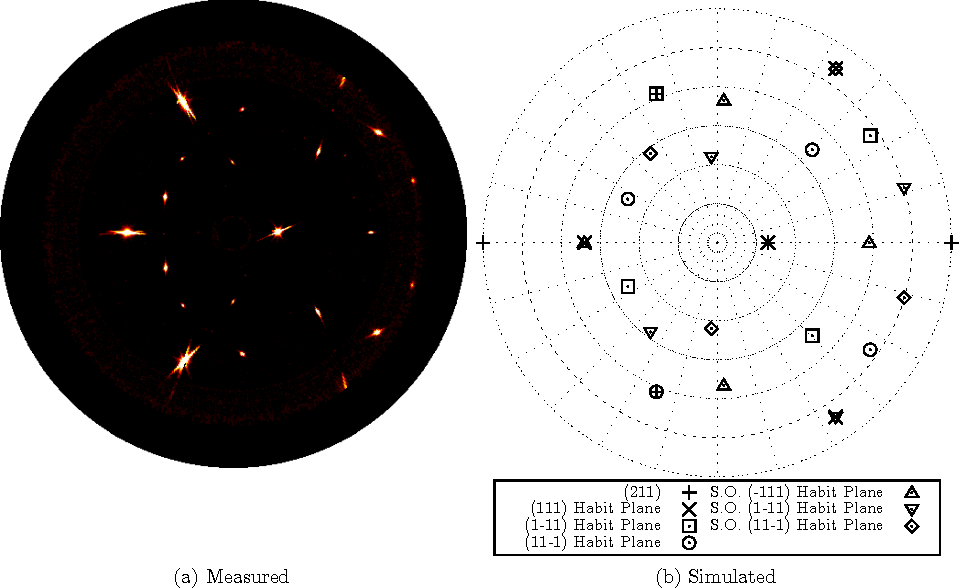
\includegraphics{211_polefigure}
\caption{\label{fig:211_polefigure}a) 2DXRD Stereographic pole figure and b) accompanying modelled pole figure, identifying the origin of each peak in the pole figure from the bulk or one of six twin variants. Overlapping peaks indicate twinning habit planes. Outermost poles are partially visible due to experimental limitations. Streaking in peaks is due to instrumental broadening. (S.O. = second-order twinning).}
\end{figure}
\section{Results}
2DXRD data was processed into a GaSb (111) pole figures as shown in FIG.~\ref{fig:211_polefigure}, representing a stereographic projection of all $<$111$>$ spacings present in the GaSb epilayer. Modeling (as per Devenyi \textit{et al.}\cite{Devenyi2011})\ of the poles present indicate that there are seven phases of GaSb, the bulk (211) orientation of GaSb and six twin variants, three first-order twins and three second-order twins from the twin variant with (111) habit plane, with 58\%, 21\% and 2\% of the intensity (and hence volume fraction) present in the twinned orientation for the films presented here. Volume fractions were determined by integration of the sum of intensity of unique (111) X-ray peaks from all twinned orientations, and divided by total intensity of all unique (111) reflections (sum of bulk and twin intensities), performed using \textit{Bruker GADDS}. There are two distinct nomenclatures used in literature to describe phases present in epitaxial films.\cite{Kim2010a,Lange1991,Johnson2011,DeLyon1995} One method describes the crystallographic direction which is normal to the surface for each phase, while the other (which the authors choose to employ here) describes the nature of the crystallographic orientation relationship between the secondary phases with respect to the orientation of the substrate. Where reference is made to literature using the first, descriptions will be translated into the second for ease of comparison.

Indexing of the crystal unit cells present in the film was performed using \textit{Bruker APEXII} single crystal refinement software, to obtain orientation matrices for the Si substrate as well as the seven GaSb phases. The bulk thin film orientation matrix was then compared to the substrate matrix and a tilt calculated using \textit{orilib} a crystal orientation calculation library, yielding a tilt of 2.65\degree, 2.55\degree and 2.40\degree $\pm$ 0.2\degree about the [01$\overline{1}$] direction towards [$\overline{1}$11], these values are indistinguishable within experimental error. The (111) habit plane twin formed in these films is also tilted with respect to the substrate, by the same angle as the bulk, this is expected by crystallography, since this twinned orientation shares extended interfaces with the bulk orientation.
\begin{figure}
    \centering
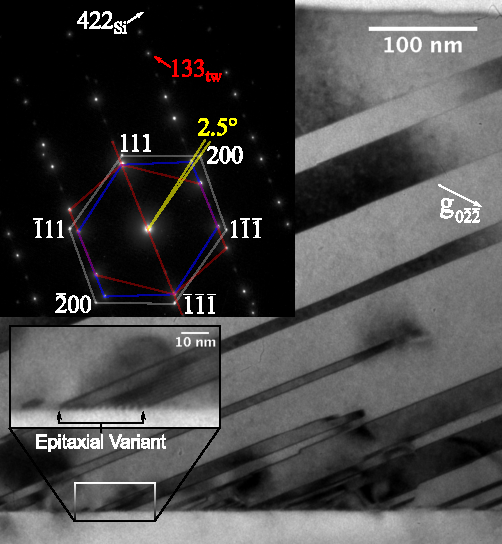
\includegraphics{211_tem}
\caption{\label{fig:211_tem}Conventional TEM image of the (0$\overline{1}$1) cross section, with inset diffraction pattern of the epitaxial and (111) habit plane twin variant in blue and red, respectively, and inset higher-magnification of the epitaxial variant showing misfit dislocations.}
\end{figure}

Two transmission electron microscopy (TEM) cross-sections were prepared, in orthogonal directions of [0$\overline{1}$1] and [1$\overline{1}\overline{1}$]. The specimens were prepared by conventional mechanical polishing and ion milling, and examined as described in Woo \textit{et al.}\cite{Woo2012} Conventional TEM imaging of the (0$\overline{1}$1) cross-section of the epilayers, combined with the selected area electron diffraction (SAED) pattern of the [0$\overline{1}$1] zone axis as shown in FIG.~\ref{fig:211_tem} confirms the presence of microtwins with (111) habit planes. These microtwins are observed in the perpendicular (1$\overline{1}\overline{1}$) cross-section as large bands lying parallel to the interface over a long-range, alternating with the epitaxial variant (not shown). The observed misorientation between the GaSb and Si reflections in the [0$\overline{1}$1] SAED pattern also indicate a tilted epilayer (both epitaxial and twin variants) with a tilt of 2.54$^\circ \pm 0.2^\circ$ towards the [$\overline{1}$11] direction. The 133 reflection of the twinned GaSb nearly coincides with the Si substrate normal 422 reflection. The GaSb twin variant can be differentiated in real space by selective dark-field imaging formed using one of the twinned reflection spots. The jagged features at the GaSb/Si interface (seen in detail in the inset of FIG.~\ref{fig:211_tem}) only belong to the epitaxial variant. This is indicative of the presence of misfit dislocations at the portions of the interface where the epitaxial region meets the substrate, as characterized by Vajargah \textit{et al.}\cite{Vajargah2011b}
\section{Discussion}
Analysis using an atomic ball-and-stick model, along with trigonometric modelling of lattice plane spacing, can be used to demonstrate that the tilted epitaxy reduces the projected in-plane lattice strain along one dimension for the GaSb/Si system. FIG.~\ref{fig:211_model} shows the alignment of planes present in the epitaxial and twinned variants of the GaSb epilayer. The Si(111) plane spacing (in red) at an angle of 19.471\degree to the Si(211) surface is aligned to the GaSb(111) plane spacing (in blue), by a tilt of 2.50\degree in the epilayer. The relationship describing zero projected strain condition between these planes across the interface is described in EQN.~\ref{eqn:211_epi} for the case of $a_{Sub} = a_{Si}$ and $a_{Film} = a_{GaSb}$, where $\delta$ is the tilt angle. This relationship (dot-dash line) also applies over the full range of common heteroepitaxial lattice mismatches grown on (211) substrates, from GaP/Si to CdTe/Si, as shown in FIG.~\ref{fig:211_data}.
\begin{gather} 
 \frac{ a_{film}}{\sqrt{3} \sin(19.471^\circ + \delta)} = \frac{a_{Sub}}{\sqrt{3}\sin(19.471^\circ)} \label{eqn:211_epi}\\
 \frac{ a_{film}}{2\sin(74.207^\circ + \delta)} = \frac{ a_{Sub}}{\sqrt{3}}   \label{eqn:211_twin}
\end{gather}
\begin{figure}
    \centering
\includegraphics{211_model}
\caption{\label{fig:211_model}Ball-and-stick atomic model of a triple junction of the epitaxial orientation, twinned orientation (with (111) habit plane in blue), and the Si(211) surface. Geometrical alignment of the atomic planes as described by EQNs.~\ref{eqn:211_epi} and \ref{eqn:211_twin} are also shown in red/blue and black, respectively. Terrace (T) and edge (E) atom labels denote the two non-equivalent surface sites.}	
\end{figure}
\begin{figure}
    \centering
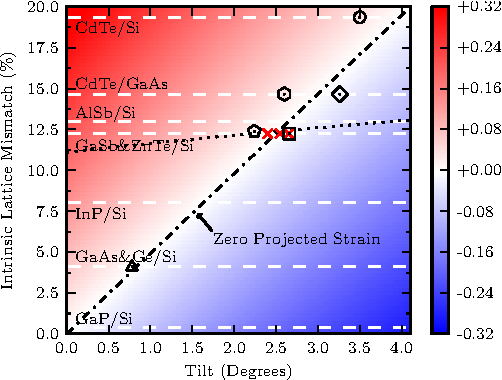
\includegraphics{211_data}
\caption{\label{fig:211_data}Colormap showing the projected strain as a function of 
intrinsic lattice mismatch and positive tilt angle of an epitaxial film, computed from 
EQN.~\ref{eqn:211_epi} with the zero projected strain contour highlighted (dot-dash 
line). The dotted line also overlays EQN.~\ref{eqn:211_twin}. Experimental data points 
from this work ($\times$), Ref.~\textcite{Zhao2011} ($\odot$), Ref.~\textcite{Wang2011a} 
($\boxdot$), Ref.~\textcite{Johnson2011} ($\Diamond$, $\bigtriangleup$) and 
Ref.~\textcite{smith2012_znte,smith2012_gaas} ($\pentagon$, $\varhexagon$) are shown, 
indicating good agreement with measured tilts of thin films. Common heteroepitaxial 
systems are also highlighted. Close lattice mismatches are merged for figure clarity.}
\end{figure}
In the twinned orientation, the Si($\overline{1}$11) plane spacing is aligned to the projection of the GaSb(200)$_{tw}$ plane spacing (both in black) onto the GaSb/Si interface, by a tilt of 2.22\degree. The geometrical constraints of these planes can be described by the relations as expressed in EQN.~\ref{eqn:211_twin}. The line of zero projected strain for the twinned region is also shown in FIG.~\ref{fig:211_data} (dotted line). The applicability of EQN.~\ref{eqn:211_twin} is considerably more limited across heteroepitaxial systems, as the constraints described by EQN.~\ref{eqn:211_epi} also needs to be simultaneously satisfied as extended interfaces are shared. However, an equivalent relationship describing another set of planes for other lattice mismatches may replace the relationship described by EQN.~\ref{eqn:211_twin}. The proposed ball-and-stick atomic model (FIG.~\ref{fig:211_model}) also shows that the Ga- and Sb-atoms in the twinned variant are perfectly registered with the terrace (T) and edge (E) atoms of the Si substrate. The epitaxial variant interface is significantly distorted, and the same atomic registration of Ga- and Sb-atoms to the underlying Si substrate does not occur, however the projected sublattice is still aligned. This correlates well with the misfit dislocations observed at the GaSb/Si interface in the inset of FIG.~\ref{fig:211_tem}.

For general case of an epilayer with unknown twin volume-fraction, the tilt is bounded by competing factors of minimizing strain in both the epitaxial and twinned variants (as in GaSb on Si), with the projected strain effectively minimized at the volume-fraction weighted average of the two tilts. For GaSb with 58\%, 21\% and 2\% twin fraction, the predicted tilts are 2.493\degree, 2.498\degree and 2.500\degree. This small variation in tilt angle is due to the steeper slope of EQN.~\ref{eqn:211_epi}, thus its contribution dominates the weighted average. The intrinsic +12.2\% lattice mismatch between GaSb and Si is minimized, however there are localized strain variations between the epitaxial and twinned regions. For a film with 58\% twin, the projected (111) d-spacing in the epitaxial region is +0.03\% (in compression), while the projected GaSb(200) and Si($\overline{1}$11) d-spacing in the twinned region is -0.12\% (in tension). Thus, the proposed driving force for the tilted epilayer during growth is the minimization of lateral strain of close-packed (111) planes (red/blue planes in FIG.~\ref{fig:211_model}), in one dimension within the two-dimensional projected interface net.

In addition to accounting for the tilt observed for GaSb on Si, this model predicts the tilts observed in several other material systems. The growth of CdTe on Si(211) and GaAs(211) is a common use to buffer the growth of HgCdTe for detector applications. Several authors\cite{Triboulet2009,Yu1999,Lange1991} published results which indicate CdTe epilayers which are tilted in the range of 3.5\degree on Si(211)\cite{Zhao2011} and 3.26\degree on GaAs(211)\cite{Johnson2011}, about the [01$\overline{1}$] direction towards [$\overline{1}$11]. The direction and magnitude reported by those authors agrees well with the tilt of 3.97\degree and 3.00\degree, respectively, as predicted by this model. Discrepancy between the predicted and reported value of tilt is expected to be partially due to the presence of twinning in the epilayer, along with uncertainty in the reported values.

ZnTe is often used as an intermediate buffer epilayer, prior to the growth of CdTe and HgCdTe on Si(211).\cite{Zhao2011,Dhar1997a} Wang \textit{et al.}\cite{Wang2011a} published results which indicate epilayer tilts in the range of 2.66\degree while Smith \textit{et al.}\cite{smith2012_znte} reports tilts of 2.24\degree. This is in good agreement to the predicted value of 2.50\degree obtained from the proposed model. The good matching between our predicted and the reported values of tilt in ZnTe on Si(211) is expected to be due to the substantially low degree of twinning observed.

The model also makes a prediction of the tilt expected from the growth of GaAs on Si(211), a value of 0.83\degree is predicted. A tilt of 0.781\degree is reported by Johnson \textit{et al.}\cite{Johnson2011} when grown alone, and 0.835\degree when capped subsequently with CdTe, again demonstrating good agreement with the model.

For the systems AlSb/Si, InP/Si and GaP/Si, the model predicts tilt angles of 2.65\degree, 1.64\degree and 0.07\degree. Measurements of these material systems are expected to yield tilts that quantitatively follow this model.
\section{Implications for Symmetry and Energy at Epitaxial Surfaces}
The natrually asymmetric (211) surface of cubic non-polar semiconductors offers a alternative route to breaking the symmetry for epitaxial growth. The (211) surface offers two unique properties which can enhance nucleation and growth of lattice mismatched thin films, it's asymmetric surface offers a energy landscape offering different bonding locations, and it's surface has a naturally stepped nature.

The two non-equivalent surface sites present on an unreconstructed (211) surface offer an energy landscape which encourages the nucleation of the polar adatoms. Such a preferred nucleation of adatoms into the two non-equivalent sites results in the natural elimination of anti-phase-domains.

The surface of (211) oriented semiconductors, in addition to having non-equivalent sites, also has a naturally asymmetric surface, consisting of 
%Other useful examples
%\textsubscript{} and \textsuperscript{} are the best way to do super/sub (provided by fixltx2e)

%\printbibliography
%\printindex
\end{document}
